\subsection{Basic Algorithm}

The basic algorithm will be to connect interested peers with one another via a DHT that stores peers lists, with the peers themselves forming together to create the DHT.
They will store only peer information on the DHT, not the blocks (content) themselves.

A peer first tries to download the file from an origin web server using traditional client-server download.  If at some point one of the following conditions occurs, the download switches to a 
peer-to-peer content delivrey (swarming download):
\begin{enumerate}
\item First, the client waits a maximum number of seconds $T$ after the start of a normal HTTP download to receive the first byte of data.  
If $T$ seconds passes without receiving any data, it transitions to a P2P download.  
This allows the system to decide quickly whether the origin server is over-burdened and switch to peer-to-peer if needed.   
\item After the client begins receiving data from the server, it monitors whether the receive rate falls below a certain fixed 
threshold of $R$ bytes per second over the last $W$ seconds.  If the receive rate ever drops below $R$, the client switches to peer-to-peer delivery.  
This is to accomodate for servers with slow connections and for file downloads that become slow mid-download.
\end{enumerate}

Should the client transition to peer-to-peer delivery, it may need to first lookup meta-data about the file (for example, the size) if it 
hasn't yet received this information.  To do so the client calculates a hash value for the URL being downloaded, and uses that as a $key$ value in the 
DHT to retrieve meta-data stored there about the file.  After determining the size, the peers chooses $b$ blocks of the file to download, and retrieves lists of peers 
who have those blocks by hashing the URI plus the block number, one list per block.  
The peer downloads the block from the peers listed.  After downloading, 
it then adds itself to the list of peers willing to share that block (see Fig. \ref{fig:download_all_steps}).  While it is attempting to retrieve the list of peers for a given block, 
it connects back to the origin server and requests the block, as a shortcut in case no peers are listed in the DHT.  If a peer downloads a file whose meta-data 
is not yet listed in the DHT, it adds that meta-data (for instance, the first time any peer downloads a file, that peer will upload information about that file to the DHT).
To combat the ``slow last block'' problem,  peers download the last block from several peers simultaneously, similar to 
BitTorrent \footnote{In reality, $b$ is more like a peer connection limit.  We download from up to $b$ peers at a time, i.e. if you have $b$ set to 10 and have 5 blocks left, 
each block will be downloaded redundantly from 2 different peers, with the last block being downloaded by 10 peers redundantly.}.

\begin{figure*}
  \begin{center}
    \subfigure[Peer downloads list of blocks]{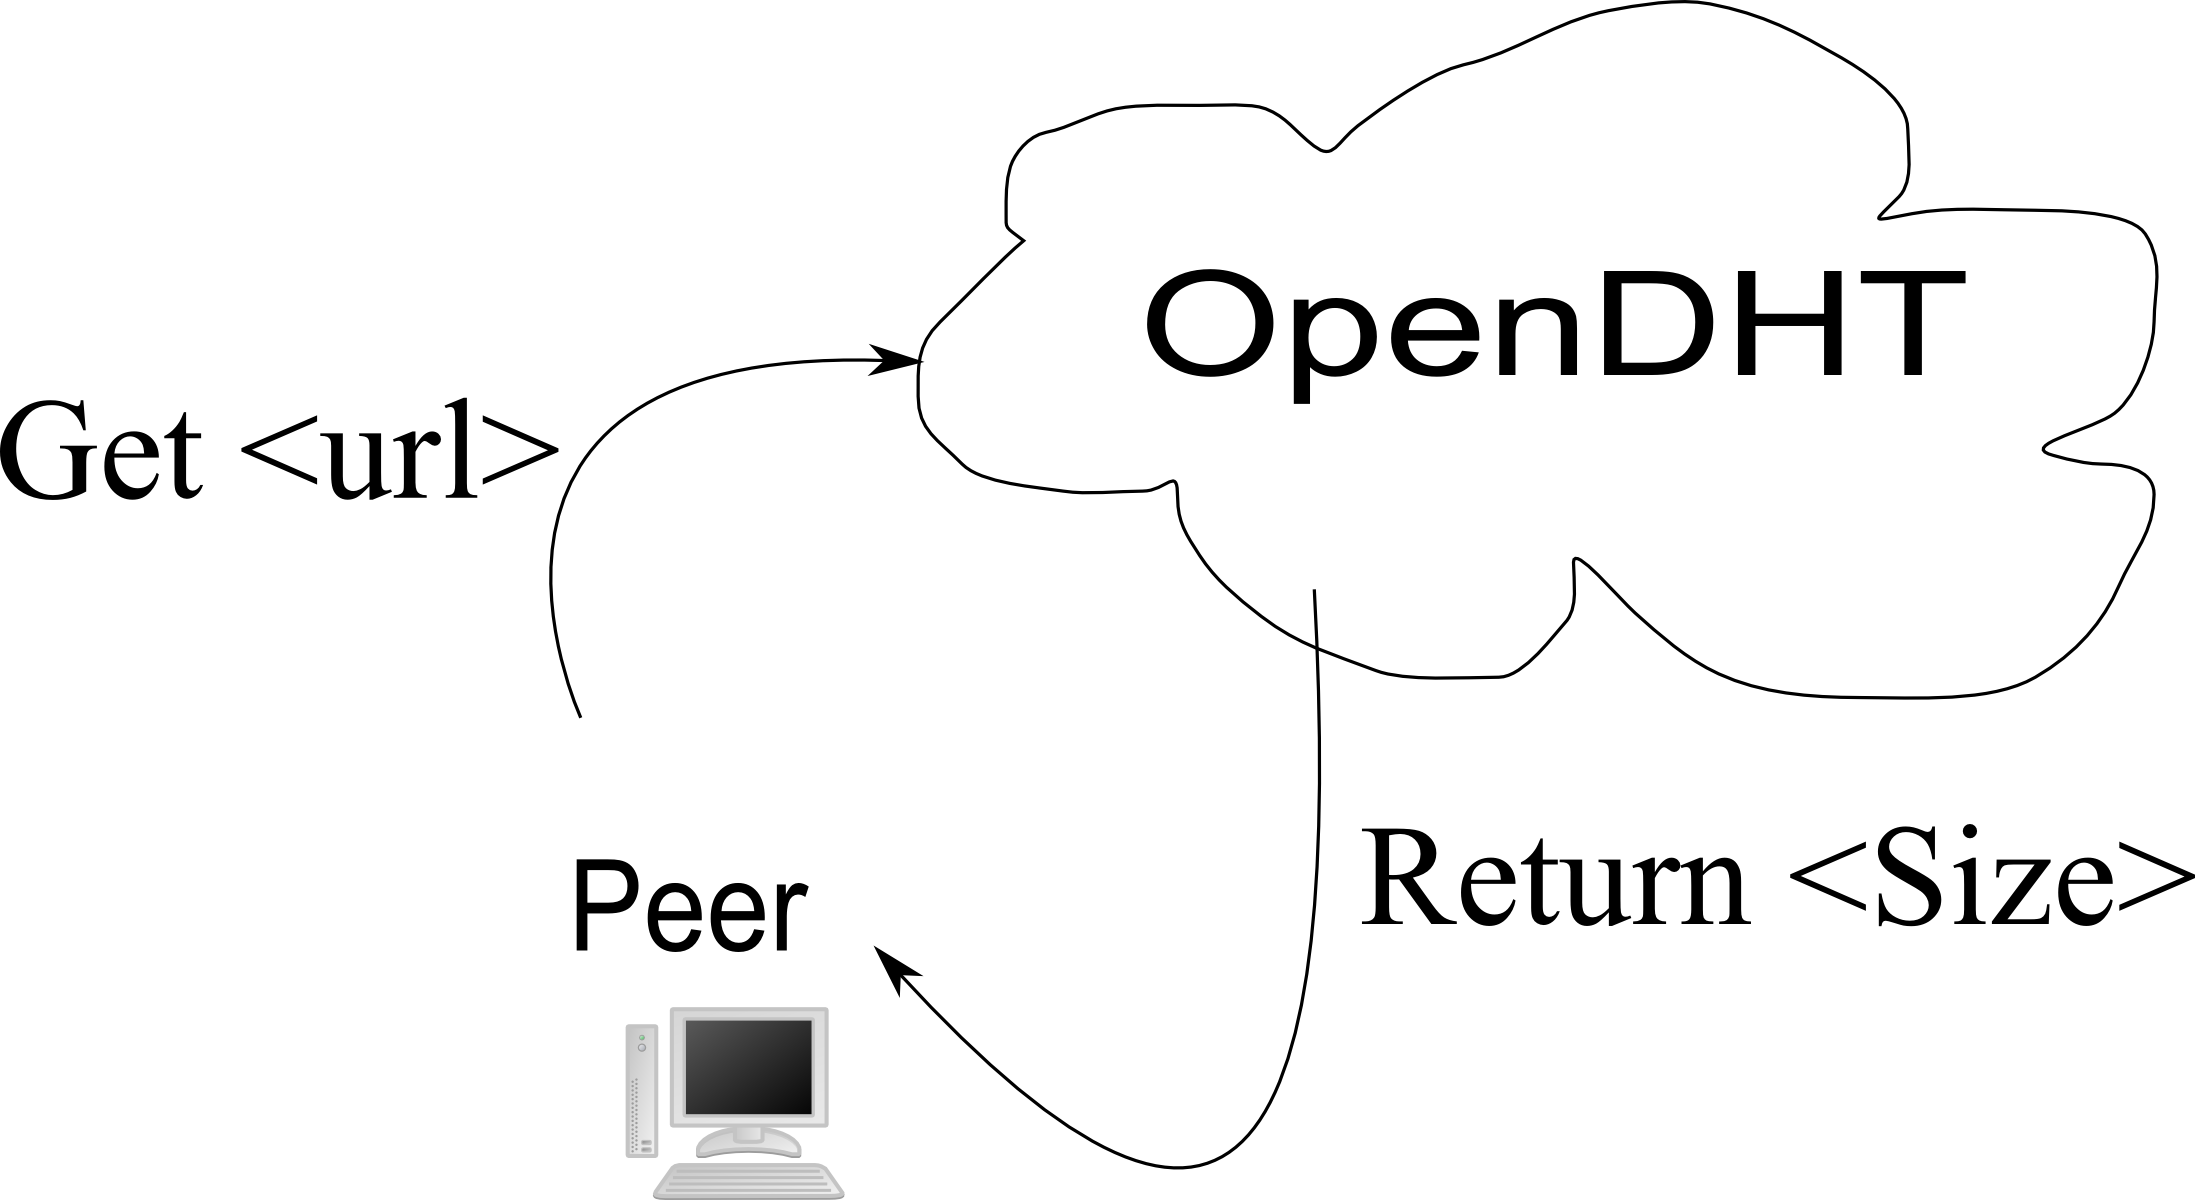
\includegraphics[width=7cm]{description_pics/peer_step_1.png}}
    \subfigure[Peer downloads a list of peers which have a block]{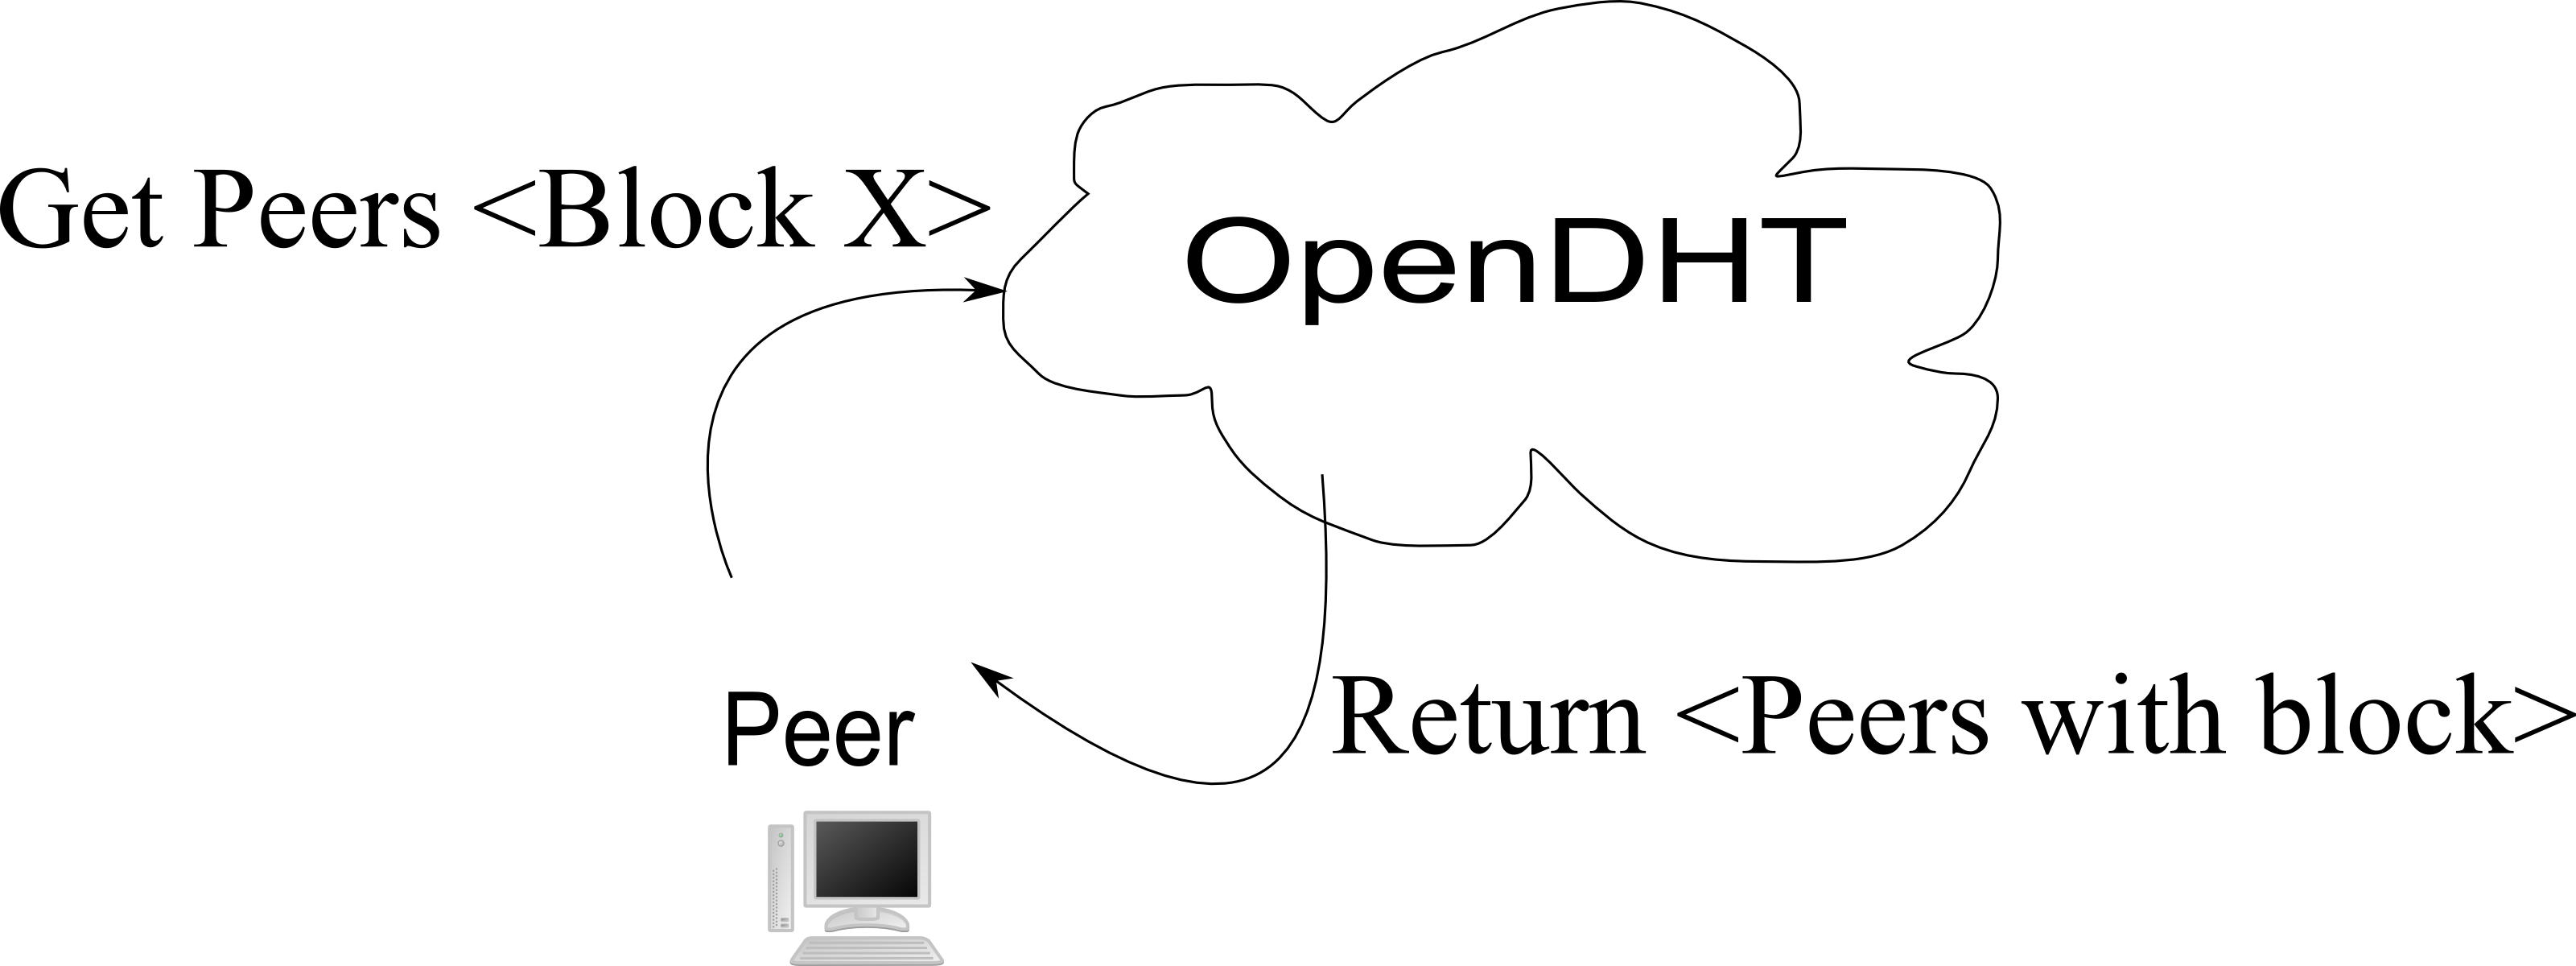
\includegraphics[width=7cm]{description_pics/peer_step_2.png}}
    \subfigure[Peer adds itself to list of peers who have that block]{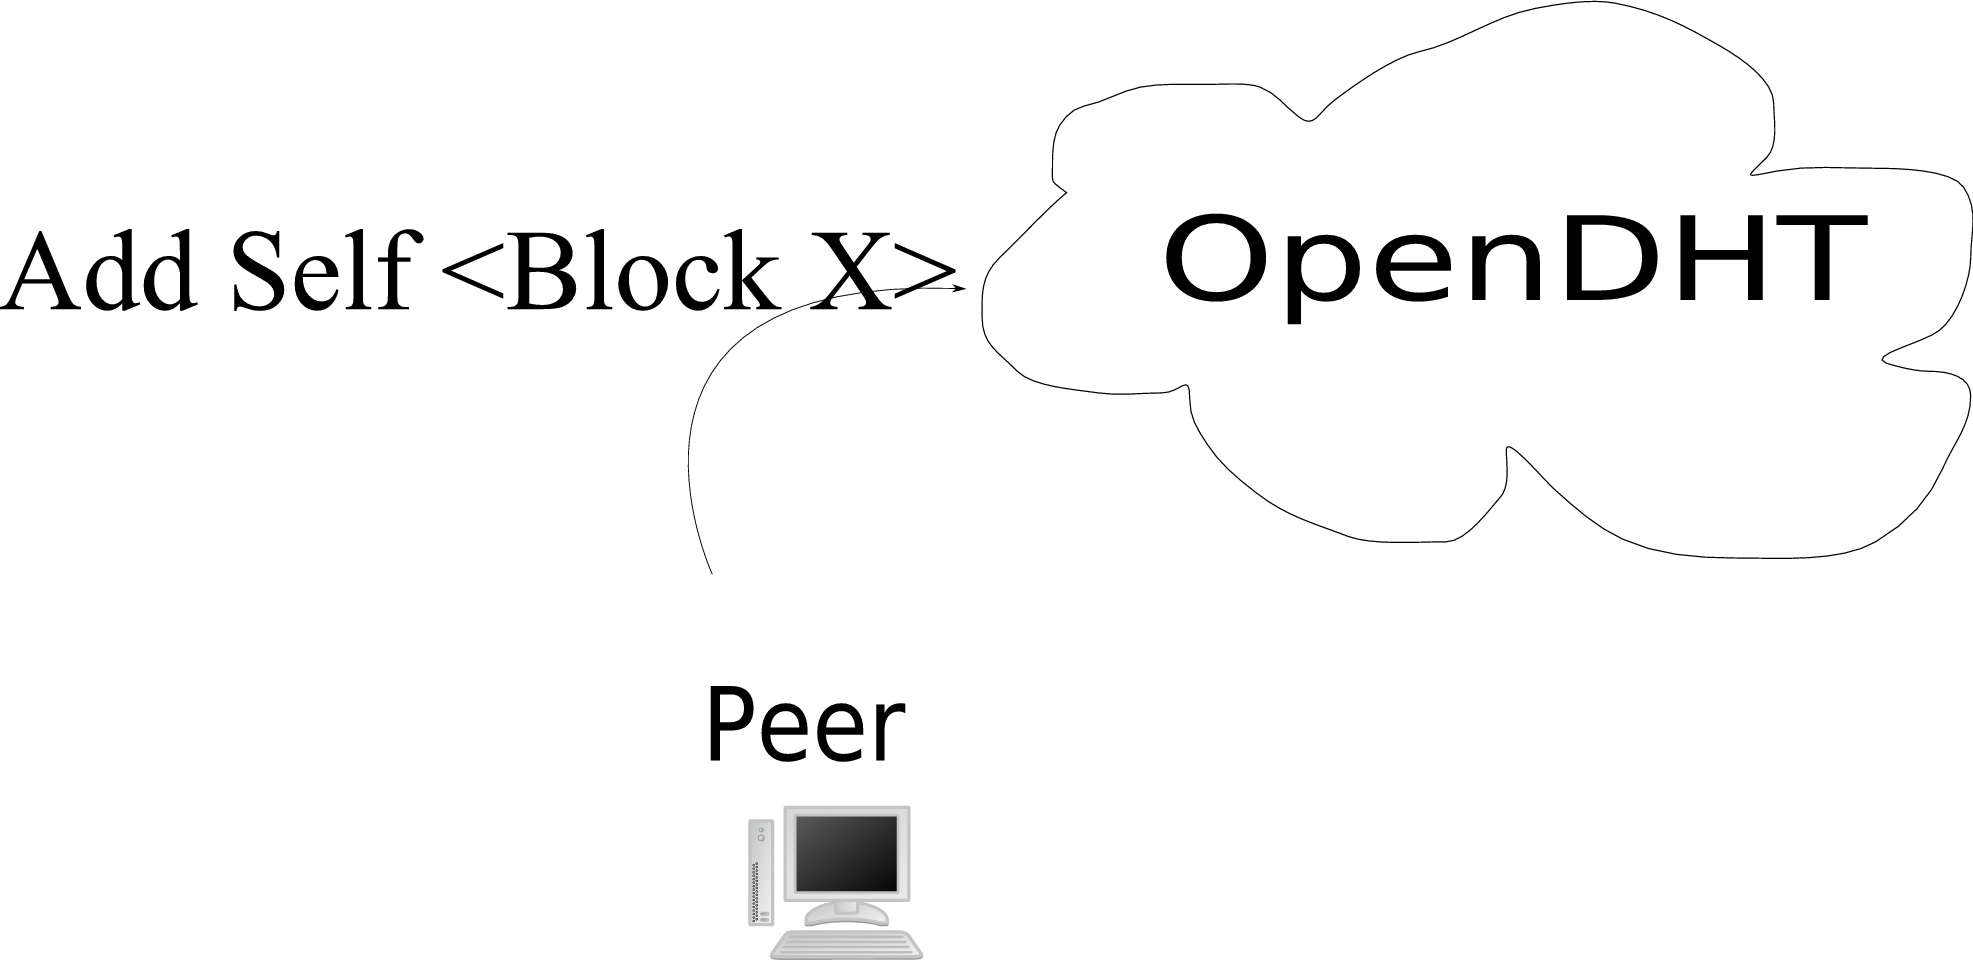
\includegraphics[width=7cm]{description_pics/peer_step_3.png}}
    \caption{Steps to accomplish a peer-to-peer-web download.}
    \label{fig:download_all_steps}
  \end{center}
\end{figure*}

